\documentclass[sn-mathphys-num]{sn-jnl}
\usepackage{graphicx}%
\usepackage{multirow}%
\usepackage{amsmath,amssymb,amsfonts}%
\usepackage{amsthm}%
\usepackage{mathrsfs}%
\usepackage[title]{appendix}%
\usepackage{xcolor}%
\usepackage{textcomp}%
\usepackage{manyfoot}%
\usepackage{booktabs}%
\usepackage{algorithm}%
\usepackage{algorithmicx}%
\usepackage{algpseudocode}%
\usepackage{listings}%
\usepackage{float}

\theoremstyle{thmstyleone}%
\newtheorem{theorem}{Theorem}
\newtheorem{proposition}[theorem]{Proposition}% 
\theoremstyle{thmstyletwo}%
\newtheorem{example}{Example}%
\newtheorem{remark}{Remark}%

\theoremstyle{thmstylethree}%
\newtheorem{definition}{Definition}%
\raggedbottom


\begin{document}

\title[Article Title]{Advancing Temporal Forecasting: A Comparative Analysis of Conventional Paradigms and Deep Learning Architectures on Publicly Accessible Datasets}

%%=============================================================%%
%% GivenName	-> \fnm{Joergen W.}
%% Particle	-> \spfx{van der} -> surname prefix
%% FamilyName	-> \sur{Ploeg}
%% Suffix	-> \sfx{IV}
%% \author*[1,2]{\fnm{Joergen W.} \spfx{van der} \sur{Ploeg} 
%%  \sfx{IV}}\email{iauthor@gmail.com}
%%=============================================================%%

\author[1]{\fnm{Liang} \sur{Gao}} \email{liang.gao@gwu.edu}

\author[1]{\fnm{Reza} \sur{Jafari}} \email{rjafari@email.gwu.edu}
% \equalcont{These authors contributed equally to this work.}

\author*[1]{\fnm{Amir H.} \sur{Jafari}}\email{ajafari@email.gwu.edu}
% \equalcont{These authors contributed equally to this work.}

\affil[1]{\orgdiv{Data Science Department}, \orgname{George Washington University}, \orgaddress{\street{725 21st St. NW}, \city{Washington}, \postcode{20052}, \state{DC}, \country{United States}}}

% \affil[2]{\orgdiv{Department}, \orgname{Organization}, \orgaddress{\street{Street}, \city{City}, \postcode{10587}, \state{State}, \country{Country}}}

% \affil[3]{\orgdiv{Department}, \orgname{Organization}, \orgaddress{\street{Street}, \city{City}, \postcode{610101}, \state{State}, \country{Country}}}



%%==================================%%
%% Sample for unstructured abstract %%
%%==================================%%

\abstract{In this study, we compare the performance of classical time series models (AR, MA, ARMA, ARIMA) and modern deep learning techniques (LSTM, Bi-LSTM, Seq2Seq) alongside a state-of-the-art Transformers model. These models have been individually studied and applied to specific problems, but the lack of a standardized benchmark for comparing their performance across diverse datasets creates a significant gap in the literature. The goal of this research is to benchmark the performance of representative time-series models across different datasets. We evaluate the models using three publicly available datasets and compare their prediction accuracy using metrics such as MSE, RMSE, and MAE. The results show that modern deep learning techniques outperform classical models, with the simplest architecture, LSTM, achieving the lowest MSE across all datasets. Although the Transformers model demonstrated superior performance compared to classical models, it did not outperform modern techniques. This suggests that for the datasets used in this study, complex Transformers architectures may not be necessary to achieve optimal results. We hope our study can provide some insights into time series studies.}

\keywords{Time series modeling, ARIMA, LSTM, Transformers}

\maketitle

\section{Introduction}\label{sec1}
Time series data refers to a sequence of data points collected or recorded at successive, equally spaced time intervals  \cite{adhikari2013introductory}. Time series modeling is a rapidly advancing field that has garnered significant attention from the research community in recent decades. The primary objective of time series modeling is to systematically collect and analyze historical data to develop a model that accurately represents the underlying structure of the series. This model is then used to predict future values or make forecasts based on the observed patterns in the data. 

Time series analysis is a critical area of research with applications spanning diverse fields, such as finance \cite{kim2011time}, social science \cite{box2014time}, climate science \cite{mudelsee2010climate}, energy management \cite{chou2018forecasting}, and healthcare \cite{gao2020time}. Numerous models have been developed to address specific problems in these domains, ranging from classical linear models like AR, MA, and ARIMA to advanced deep learning architectures such as LSTM and Transformers. 

The Autoregressive(AR) model has been employed to predict the instantaneous phase and frequency of neural oscillations in EEG data, demonstrating its effectiveness in real-time forward prediction for shorter intervals \cite{shakeel2020time}. Researchers have utilized the Autoregressive Moving Average (ARMA) model in combination with the Levenberg-Marquardt algorithm for speech recognition applications, demonstrating its effectiveness in handling time series data in this domain \cite{jafari2024speech}. As demonstrated in the study by \cite{chimmula2020time}, the LSTM network was used to forecast the COVID-19 outbreak in Canada, predicting trends, potential stopping points, and multi-day case counts. As discussed by \cite{jin2022time}, the authors proposed a method using a Time Series Transformer (TST) to recognize fault modes in rotating machinery. They combined the TST with a time series tokenizer and demonstrated its superior fault identification capability compared to traditional CNN and RNN models.

However, there is a noticeable lack of benchmarking studies comparing these models' performances on standardized datasets. The primary objective of this study is to evaluate and compare the performance of classical time series models \cite{box2015time}—Autoregressive(AR), Moving Average (MA), Autoregressive Moving Average (ARMA), and Autoregressive Integrated Moving Average (ARIMA), advanced modern techniques, including Long Short-Term Memory (LSTM) \cite{hochreiter1997lstm}, Bidirectional LSTM (BiLSTM) \cite{graves2005framewise}, sequence-to-sequence architectures \cite{sutskever2014seq2seq}, and the state-of-the-art Transformer model \cite{vaswani2017attention}. We implemented these models across three different datasets, and multiple performance metrics, such as Mean Squared Error (MSE) and Root Mean Squared Error (RMSE), are employed to ensure a robust and comprehensive evaluation. Our study provides a quantitative foundation for assessing the accuracy and reliability of each model across the datasets. Through this analysis, we have identified the strengths and limitations of the models in three different datasets, which can offer insights into their applicability for diverse time series forecasting challenges.

\section{Methodology}
\subsection{Data}
We utilized three public and realistic datasets in this study to evaluate the performance of various time series models:
\begin{itemize}
    \item \textbf{Weather Station Beutenberg Dataset} \cite{weather2020}: This dataset contains meteorological measurements, such as temperature, humidity, and wind speed, recorded every 10 minutes, capturing fine-grained temporal variations in environmental conditions. The data was accessed from Kaggle, and the target variable is the temperature in Celsius. 
    
    \item \textbf{Power Consumption of Tetouan City} \cite{power_consumption_of_tetouan_city_849}: This dataset comprises the energy consumption data of Tetouan City, recorded at 10-minute intervals,  offering detailed observations of energy usage patterns. It offers insights into power usage patterns and facilitates the evaluation of energy forecasting models. The dataset was retrieved from the UCI Machine Learning Repository and used to forecast the power consumption in Zone 1.
    
    \item \textbf{Air Pollution Forecasting Dataset} \cite{kaggle_lstm_dataset}: This dataset includes hourly measurements of air pollutants along with meteorological features, providing insights into atmospheric quality over time. It serves as a multivariate time series dataset to assess forecasting models in pollution monitoring. The data was sourced from Kaggle, and the target variable is the pollution called PM2.5 concentration.
\end{itemize}

\subsection{Models}

\textbf{Classical models.} We implemented four classical models: Autoregressive (AR), Moving Average (MA), Autoregressive Moving Average (ARMA), and Autoregressive Integrated Moving Average (ARIMA) models.

In an AR model, we forecast the variable of interest using a linear combination of past values of the variable.
An AR process of order \( n_a \) AR(\( n_a \))  can be written as:
\[
y(t) + a_1 y(t-1) + a_2 y(t-2) + \dots + a_{n_a} y(t-{n_a}) = \epsilon(t)
\]
Rather than using past values of the forecast variable in a
regression, an MA model uses past forecast errors. A MA process of order order \( n_b \), (MA(\( n_b \))) can be represented as:
\[
y(t) = \epsilon(t) + b_1 \epsilon(t-1) + b_2 \epsilon(t-2) + \dots + b_{n_b} \epsilon(t - n_b)
\]
The ARMA model is the combination of AR and MA models, which can be represented as:
\[
y(t) + a_1 y(t-1) + a_2 y(t-2) + \dots + a_{n_a} y(t-{n_a}) = \epsilon(t) + b_1 \epsilon(t-1) + b_2 \epsilon(t-2) + \dots + b_{n_b} \epsilon(t - n_b)
\]
Compared to pure AR and MA models, the ARMA models offer an efficient linear approach for modeling stationary time series. 
The ARIMA model is a generalization of the ARMA model with differencing, designed to handle non-stationary time series sequences. In the general form, the ARIMA(\(n_a, d, n_b\)) model can be written as:
$$
\left(1+a_1 q^{-1}+\dots+a_{n_a} q^{-n_a}\right)\left(1-q^{-1}\right)^d y(t) = \left(1+b_1 q^{-1}+\dots+b_{n_b} q^{-n_b}\right)\epsilon(t)$$
Notation:
\begin{itemize}
    \item \( y(t) \) is the value of the time series at time \( t \),
    \item \( a_1, a_2, \dots, a_{n_a} \) are the coefficients of the AR model,
    \item \( n_a \) is the order of the autoregressive model,
    \item \( b_1, b_2, \dots, b_{n_b} \) are the coefficients of the MA model,
    \item \( n_b \) is the order of the moving average model,
    \item \( \epsilon(t) \) is a white noise (WN $\sim (0, \sigma_\epsilon^2)$),
    \item \( d \) is the number of non-seasonal order differencing.
\end{itemize}

\textbf{Modern techniques.}
Three modern techniques are implemented: Long Short-Term Memory (LSTM), Bidirectional Long Short-Term Memory (BiLSTM), and Sequence-to-sequence (Seq2Seq) models. 
LSTM, introduced by Hochreiter and Schmidhuber in 1997 \cite{hochreiter1997lstm}, is a specialized Recurrent Neural Network (RNN) designed to capture long-term dependencies in sequential data while mitigating the vanishing gradient problem \cite{medsker2001recurrent}. Its architecture incorporates a cell state and three gates—input, forget, and output—to regulate information flow, making it well-suited for time series forecasting and natural language processing tasks. BiLSTM extends LSTM by processing data bidirectionally, utilizing forward and backward LSTMs to capture past and future context, which enhances its performance in tasks like time series forecasting, NLP, and speech recognition \cite{graves2005framewise}. Seq2Seq models transform input sequences into output sequences of varying lengths and are widely used in tasks such as language translation and time series forecasting. The implemented Seq2Seq architecture adopts an encoder-decoder LSTM framework enhanced by an attention mechanism inspired by Bahdanau et al. \cite{bahdanau2014neural}.

\textbf{State-of-the-Art Models.}The Transformer model, introduced by Vaswani et al. \cite{vaswani2017attention}, revolutionized deep learning with its attention mechanism and parallelized architecture. Unlike sequential recurrent models, Transformers process entire sequences simultaneously, efficiently capturing long-term dependencies. The model comprises an encoder, which applies self-attention and feed-forward layers to process input sequences, and a decoder, which generates outputs by attending to the encoder’s representation and prior outputs.

\subsection{Analysis}
This study used time series domain knowledge, including ACF/PACF plots and generalized partial autocorrelation (GPAC), to help determine the order for classical time series linear models. Besides domain knowledge, we also used a hyperparameter optimization framework - Optuna, in the experiment. These tools are introduced below. 

The Autocorrelation Function (ACF) and Partial Autocorrelation Function (PACF) are essential tools in time series analysis \cite{box2015time, hyndman2018forecasting, chatfield2019analysis}. The ACF quantifies the correlation between a time series and its lagged values, aiding in identifying trends, seasonality, and the order of Moving Average (MA) models. Significant autocorrelations at specific lags suggest predictability at those intervals. The PACF extends this by isolating the correlation between a series and its lagged values, removing the influence of intermediate lags, and making it particularly effective for determining the order of Autoregressive (AR) models.

The Generalized Partial Autocorrelation (GPAC) is used in time series analysis, particularly in Auto-Regressive Moving-Average (ARMA) modeling. It is used to estimate the order of the ARMA model when the auto-regressive (AR) and moving-average (MA) orders (\( n_a \) and \( n_b \), respectively) are not known prior. The pattern observed in the GPAC table, where a column has constant values and a row consists entirely of zeros, identifies the orders of \( n_a \) for the AR component and \( n_b \) for the MA component. Specifically, the row number represents the MA order, while the column number indicates the AR order. This structure provides a systematic approach to determining the appropriate parameters for ARMA modeling.


In addition to using time series domain knowledge (ACF/PACF plots and the GPAC table), we applied Optuna, an open-source hyperparameter optimization framework \cite{akiba2019optuna}, to determine the order of classical linear time series models. Optuna employs Bayesian optimization and pruning techniques to efficiently search for optimal hyperparameters, making it a flexible and computationally efficient tool for model tuning.

\section{Experiment results}

\subsection{Experiment settings}
Our experiments utilized AWS cloud resources to meet the computational demands of the models. Classical time series models (AR, MA, ARMA, ARIMA) were executed on AWS CPU instances due to their lightweight nature, while deep learning models (LSTM, BiLSTM, Seq2Seq, Transformer) leveraged GPU instances for efficient training and faster convergence. Standardized hyperparameters (Table \ref{tab:hyperparams}) were applied consistently across all modern and state-of-the-art models to ensure comparability.
\begin{table}[]
\centering
\begin{tabular}{lc}
\hline
\textbf{Hyperparameter} & \textbf{Value} \\ \hline
Sequence Length         & 6              \\ 
Batch Size              & 128            \\ 
Optimizer               & Adam           \\ 
Training Epochs         & 100            \\ 
Learning Rate           & 0.001          \\ \hline
\end{tabular}
\caption{Hyperparameters for LSTM, Bi-LSTM, Seq2Seq, and Transformer.}
\label{tab:hyperparams}
\end{table}

For the modern techniques (LSTM, BiLSTM, Seq2Seq), we standardized the hyperparameters using a single layer and a hidden size 2 across all models. This uniform configuration was chosen to maintain comparability and isolate the model architecture's effect on performance. In the Optuna setting, we capped the maximum order for the AR process at 20, the MA process at 10, and conducted 30 optimization trials. 
We used the drift method in the temperature dataset to fill the 9 missing values. There are no missing values in the other two datasets. Each dataset was split into 80\% for training and 20\% for validation, ensuring a balanced trade-off between model training and validation. Additionally, data was normalized to ensure fair comparison across datasets before calculating evaluation metrics using min-max scaling in Equation \ref{nomalize}.

\begin{equation}
\text{X}_{\text{normalized}} = \frac{\text{X} - \text{X}_{\min}}{\text{X}_{\max} - \text{X}_{\min}}
\label{nomalize}
\end{equation}

\subsection{Results and discussion}
In this study, we analyzed the characteristics of three datasets and systematically investigated the performance of various models on these datasets. In the following sections, we comprehensively discuss our findings and insights.

\textbf{Exploratory Data Analysis (EDA).} We conducted EDA to examine dataset characteristics and identify underlying patterns. Visualizations included sequence plots for trend observation, rolling mean and variance plots for stationarity assessment, ACF/PACF plots for model order identification and time series decomposition to analyze seasonal, trend, and residual components. Figure \ref{fig:eda_plot} presents these visualizations.
\begin{figure}[]
	\begin{center}
		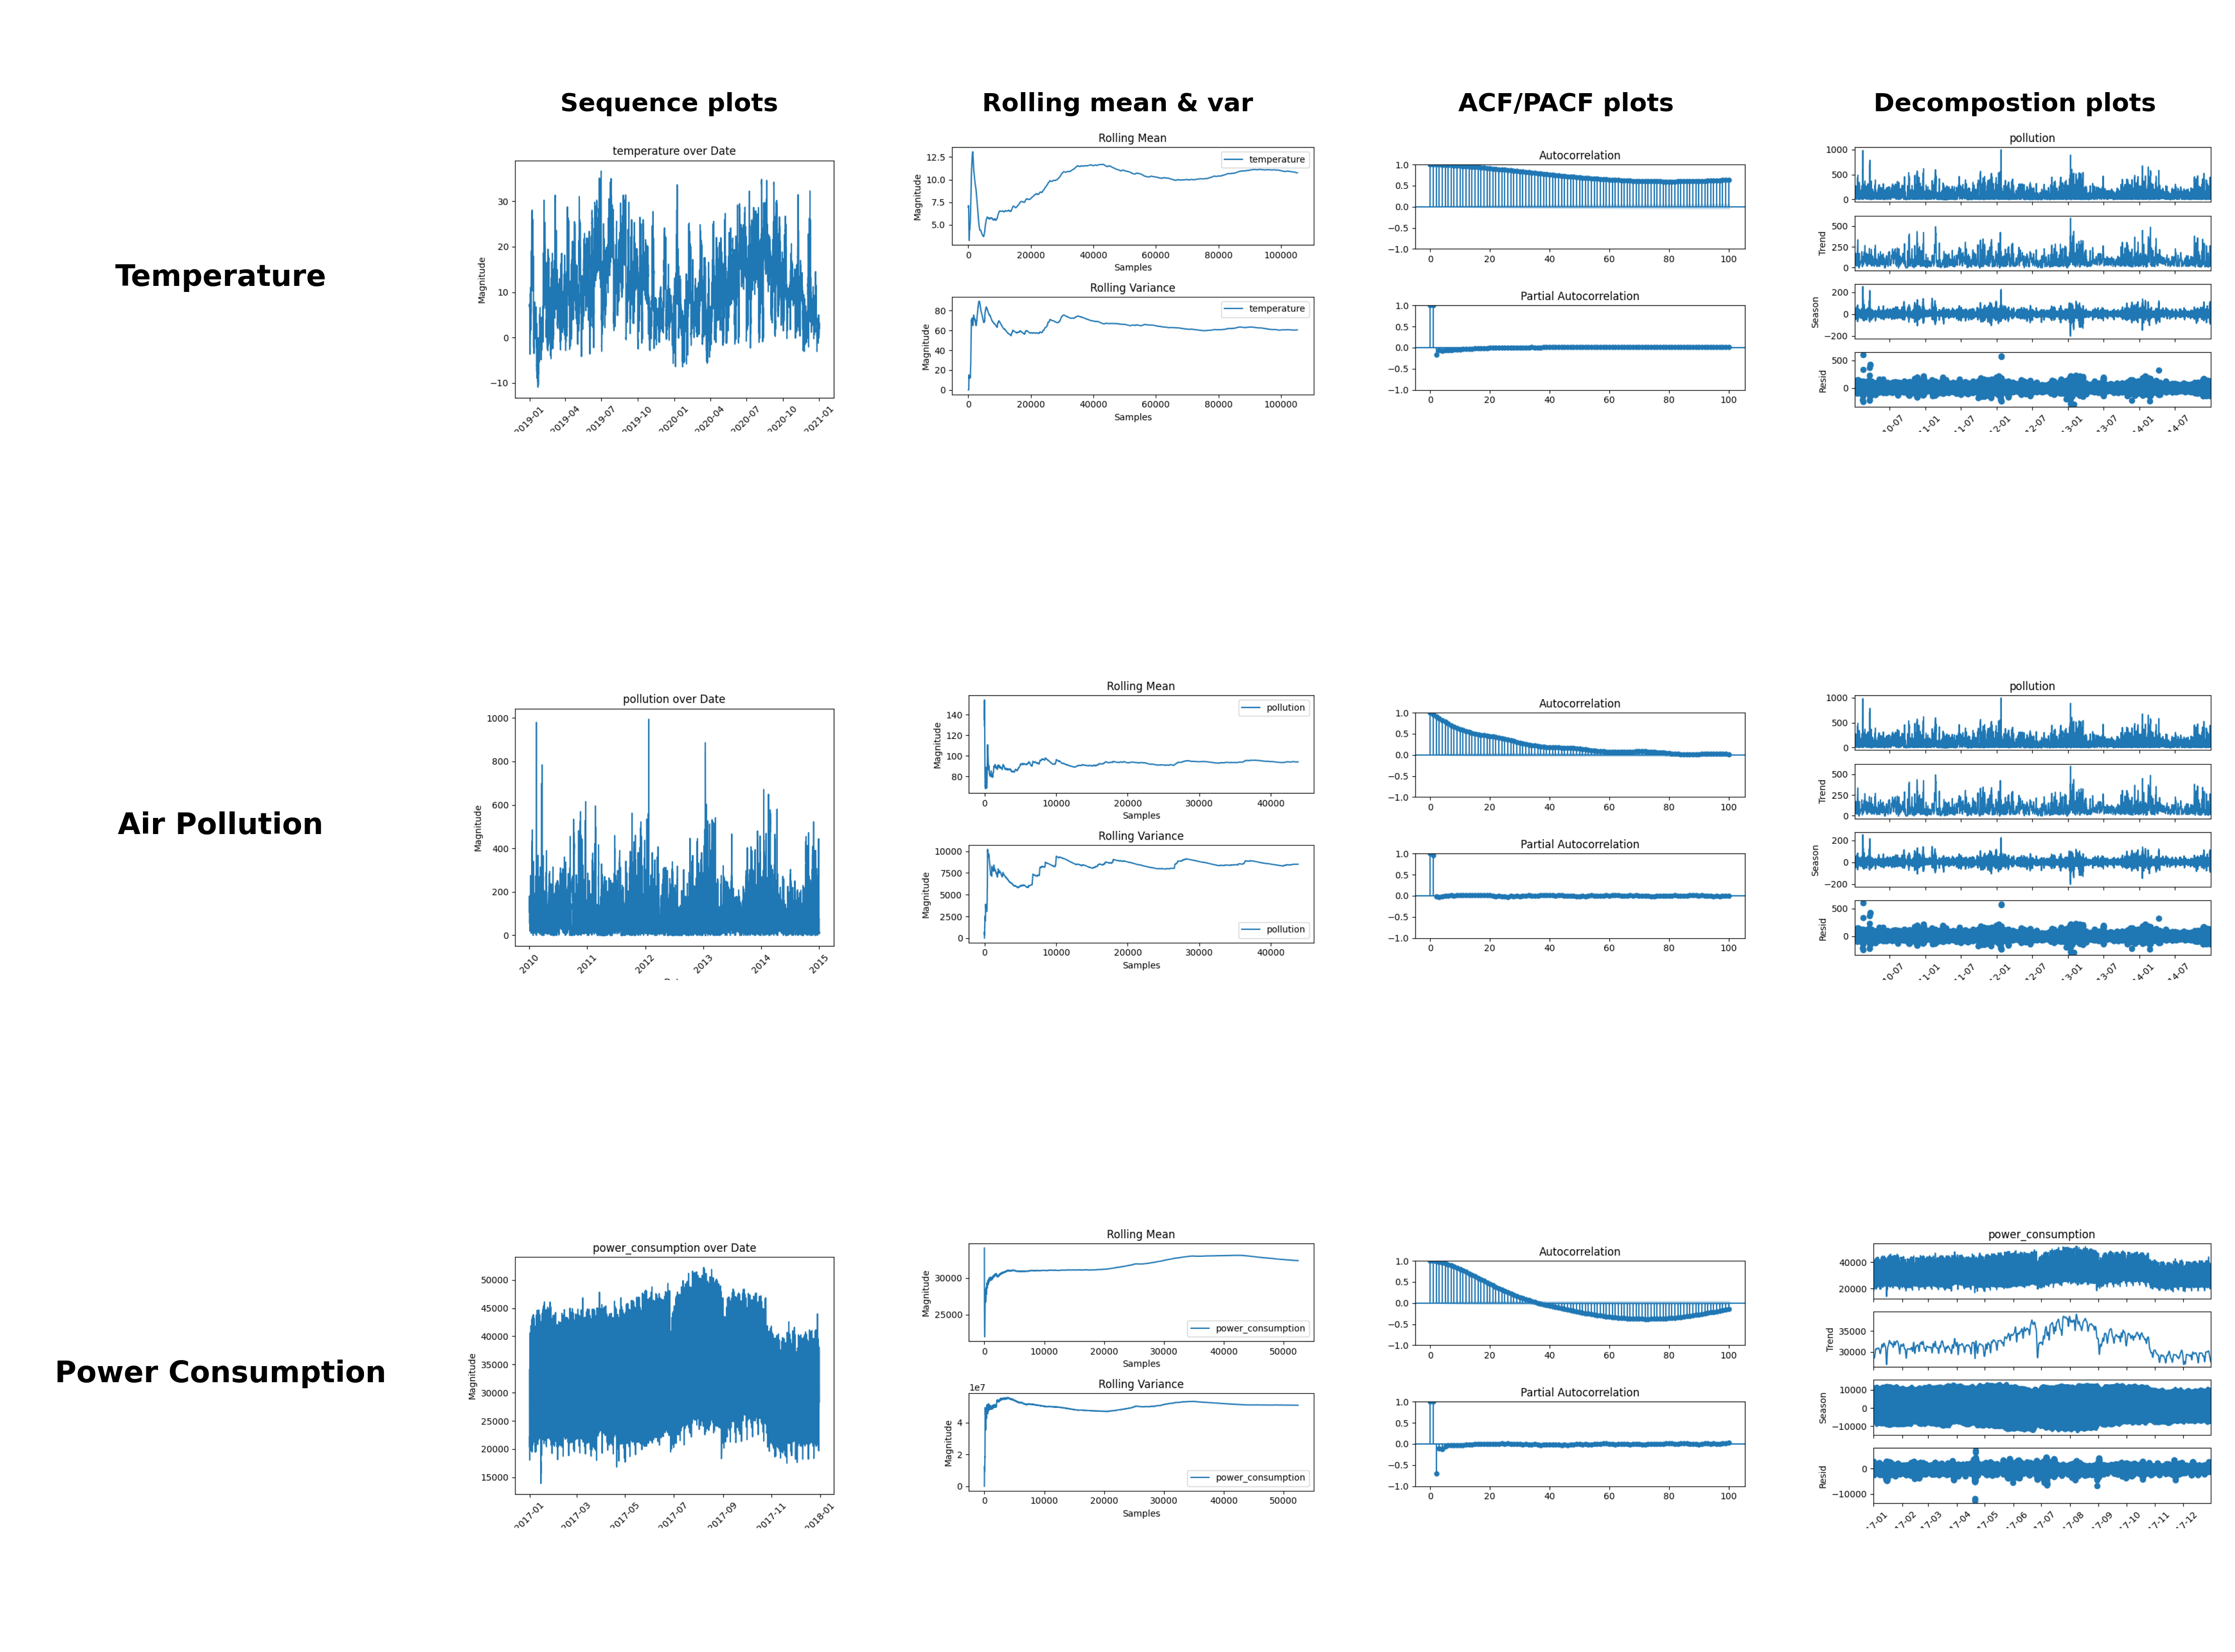
\includegraphics[scale=0.7]{sn-article-template/eda.pdf}
	\end{center}
	\caption{EDA plots: time series sequences over time, ACF\&PACF, and time series decomposition plots for three datasets.}
	\label{fig:eda_plot}
\end{figure}
All three datasets exhibited stationarity, confirmed by stable rolling means and variances. ACF tail-offs and PACF cut-offs indicated AR patterns. Table~\ref{tab:trend_seasonality} summarizes the trend and seasonality strengths: the Weather dataset showed a strong trend (94.33\%) and moderate seasonality (74.79\%), the Air Pollution dataset revealed a notable trend (86.01\%) but weak seasonality (40.67\%), and the Power Consumption dataset demonstrated both strong trend (92.41\%) and seasonality (98.64\%). 
\begin{table}[h]
\centering
\begin{tabular}{lcc}
\hline
\textbf{}        & \textbf{Strength of Trend (\%)} & \textbf{Strength of Seasonality (\%)} \\ \hline
Weather                 & 94.33                          & 74.79                                 \\ 
Air Pollution           & 86.01                          & 40.67                                 \\ 
Power Consumption       & 92.41                          & 98.64                                 \\ \hline
\end{tabular}
\caption{Strength of Trend and Seasonality for Each Dataset.}
\label{tab:trend_seasonality}
\end{table}

\textbf{Classical models.} We implemented four classical linear time series models: AR, MA, ARMA, and ARIMA, each addressing different temporal dependencies in time series data. To determine the appropriate model orders \(n_a\) for the AR component and \(n_b\) for the MA component, we used ACF and PACF plots to identify lag relationships and the GPAC table to assess lag patterns systematically. 

For the AR model, the order was set based on the cutoff in the PACF plot, while for the MA model, since there was no MA pattern from ACF and PACF plots, we used Optuna to optimize the best order, with the maximum order set to 10. The GPAC table in Figure \ref{fig:gpac1}  was used to determine the AR and MA orders for the ARMA model. We applied first-order differencing to our data for the ARIMA model, analyzing the differenced data using the GPAC in figure \ref{fig:gpac2} to identify the AR and MA orders.
\begin{figure}[H]
	\begin{center}
		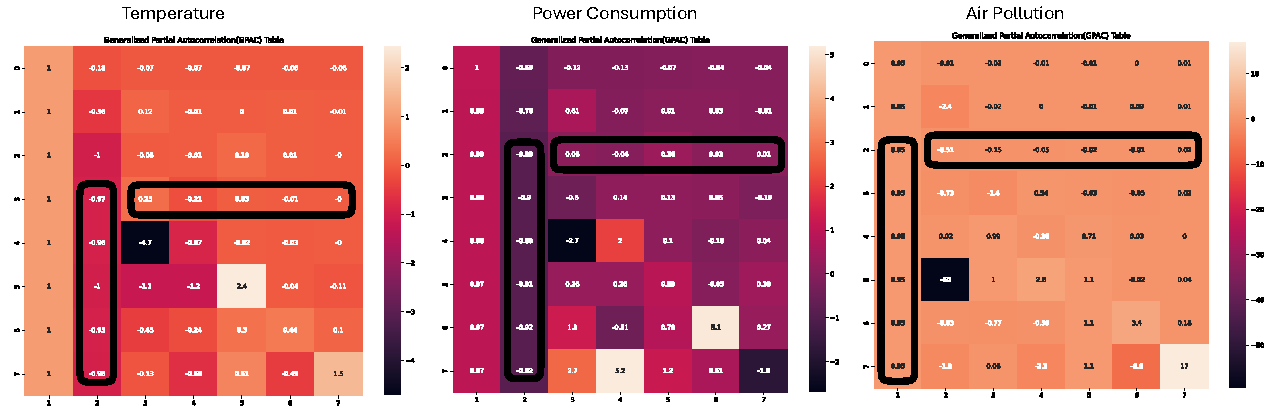
\includegraphics[scale=0.6]{sn-article-template/gpac1.pdf}
	\end{center}
	\caption{GPAC for three stationary raw datasets to find potential order for ARMA process.}
	\label{fig:gpac1}
\end{figure}

\begin{figure}[H]
	\begin{center}
		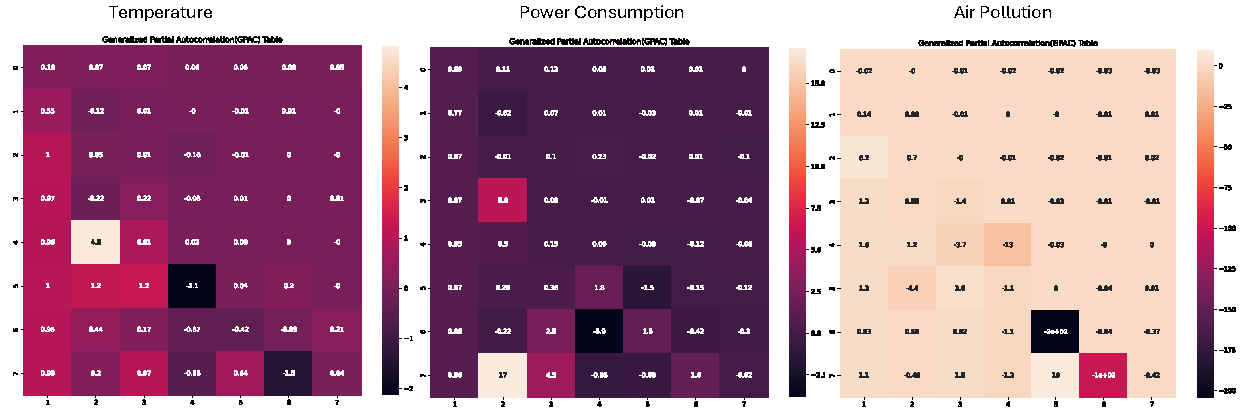
\includegraphics[scale=0.6]{sn-article-template/gpac2.pdf}
	\end{center}
	\caption{GPAC for three non-seasonal first-order differencing data to find potential order for ARMA process.}
	\label{fig:gpac2}
\end{figure}

In addition to traditional methods like domain expertise and manual plot interpretation, we utilized Optuna, an advanced machine learning optimization algorithm, for hyperparameter tuning. Optuna's efficient search strategies helped minimize errors and improve model performance. For the AR component, we set the maximum potential order to 20 and 10 for the MA component, as no clear MA pattern was found in the ACF and PACF plots. We conducted 20 trials for the AR model, 10 for the MA model, and 30 for the ARMA and ARIMA models.

Table \ref{tab:optuna} compares the model orders obtained through domain knowledge and Optuna and their respective MSE values. The minor differences in MSE suggest that while domain knowledge is valuable, Optuna offers a systematic and automated alternative, particularly when prior knowledge is insufficient or when determining an appropriate order is challenging.
\begin{table}[h]
\centering
\begin{tabular}{@{}lcccc@{}}
\toprule
\textbf{}               & \textbf{Domain Order}           & \textbf{MSE}     & \textbf{Optuna Order} & \textbf{MSE}     \\ \midrule
\textbf{AR}             &                                 &                  &                       &                  \\
Temperature             & (2)                             & 0.038986         & (4)                   & 0.038950         \\
Power Consumption       & (2)                             & 0.059108         & (10)                  & 0.059213         \\
Air Pollution           & (1)                             & 0.019484         & (5)                   & 0.019482         \\ \midrule
\textbf{MA}               &                                 &                  &                       &                  \\
Temperature             & --                              & --               & (10)                  & 0.038870         \\
Power Consumption       & --                              & --               & (10)                  & 0.059218         \\
Air Pollution           & --                              & --               & (10)                  & 0.019472         \\ \midrule
\textbf{ARMA}             &                                 &                  &                       &                  \\
Temperature             & (2,3)                           & 0.038971         & (8,2)                 & 0.038892         \\
Power Consumption       & (2,2)                           & 0.059206         & (4,5)                 & 0.059281         \\
Air Pollution           & (1,2)                           & 0.019483         & (2,6)                 & 0.019458         \\ \midrule
\textbf{ARIMA}            &                                 &                  &                       &                  \\
Temperature             & (1,1,1)                         & 0.049111         & (7,1,6)               & 0.044493         \\
Power Consumption       & (1,1,2)                         & 0.055292         & (11,1,6)              & 0.055068         \\
Air Pollution           & (4,1,5)                         & 0.019482         & (13,1,10)             & 0.019479         \\ \bottomrule
\end{tabular}
\caption{MSE comparison between models which orders determined by domain knowledge and Optuna. Predictions and ground truth are normalized using the equation in \ref{nomalize}.}
\label{tab:optuna}
\end{table}
We selected the order with the lowest MSE from those determined using domain knowledge and Optuna as the final order for each model. In cases where the GPAC showed multiple patterns, we chose the order corresponding to the lowest MSE. To evaluate the performance of the four classical models, we computed MSE, RMSE, and MAE, with results presented in Table \ref{tab:classical_metric}. The comparison between predicted and actual values is visualized in Figure \ref{fig:classical_perf}. The performance of the classical models was not very satisfactory, which is expected given their simplicity and reliance on basic approaches, primarily serving as baseline references.
\begin{table}[]
\centering
\begin{tabular}{@{}lccc@{}}
\toprule
\textbf{}               & \textbf{MSE} & \textbf{RMSE} & \textbf{MAE} \\ \midrule
\textbf{AR}             &              &               &              \\
Temperature             & 0.038950     & 0.197359      & 0.161282     \\
Power consumption       & 0.059108     & 0.243121      & 0.204268     \\
Air pollution           & 0.019482     & 0.139578      & 0.101504     \\ \midrule
\textbf{MA}             &              &               &              \\
Temperature             & 0.038870     & 0.197156      & 0.160967    \\
Power consumption       & 0.059218     & 0.243347      & 0.204480     \\
Air pollution           & 0.019472     & 0.139542      & 0.101515     \\ \midrule
\textbf{ARMA}           &              &               &              \\
Temperature             & 0.038892     & 0.197210      & 0.161051     \\
Power consumption       & 0.059206     & 0.243322      & 0.204456     \\
Air pollution           & 0.019458     & 0.139493      & 0.101845      \\ \midrule
\textbf{ARIMA}          &              &               &              \\
Temperature             & 0.044493     & 0.210933      & 0.178464     \\
Power consumption       & 0.055068     & 0.234666      & 0.193346     \\
Air pollution           & 0.019479     & 0.139569      & 0.101566       \\ \bottomrule
\end{tabular}
\caption{Performance metrics comparison for AR, MA, ARMA, ARIMA. Predictions and ground truth are normalized using the Equation \ref{nomalize}.}
\label{tab:classical_metric}
\end{table}

\begin{figure}[]
	\begin{center}
		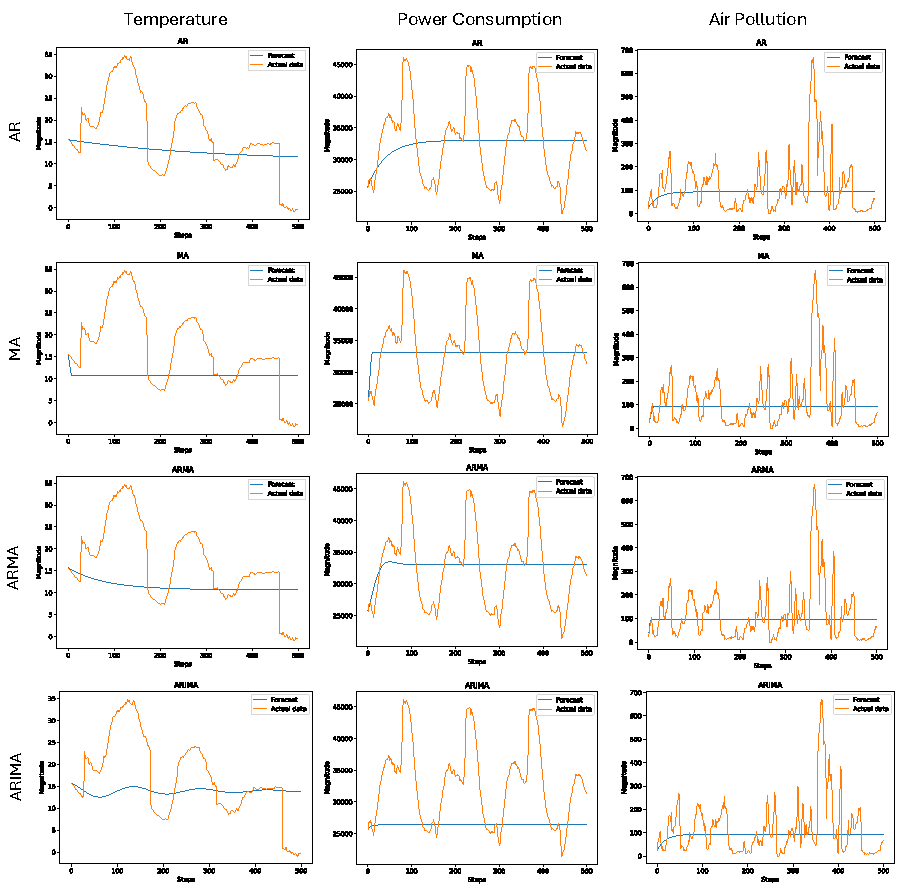
\includegraphics[scale=0.8]{sn-article-template/classical.pdf}
	\end{center}
	\caption{Plots: comparison between predicted values vs. ground truth for four classical models (AR, MA, ARMA, ARIMA) across three datasets.}
	\label{fig:classical_perf}
\end{figure}

\textbf{Modern techniques.} 
We implemented three modern techniques, including LSTM, Bi-LSTM, and Seq2Seq models. The three modern techniques were trained with identical hyperparameters, as shown in Table \ref{tab:hyperparams}, ensuring direct comparability across models and isolating the impact of each model's architecture. MSE, RMSE, and MAE were calculated to evaluate performance, as summarized in Table \ref{tab:lstm_metric}. Figure \ref{fig:modern} compares the predicted and actual values for LSTM, BiLSTM, and Seq2Seq models. The modern techniques significantly outperformed the classical models, with lower MSE values and superior accuracy. Among them, the LSTM model, despite its simplicity, achieved the lowest MSE, indicating its effectiveness for the datasets in this study.

\begin{table}[h]
\centering
\begin{tabular}{@{}lccc@{}}
\toprule
\textbf{}               & \textbf{MSE} & \textbf{RMSE} & \textbf{MAE} \\ \midrule
\textbf{LSTM}           &              &               &              \\
Temperature             & 0.000127     & 0.011277      & 0.004017     \\
Power consumption       & 0.000175     & 0.013225      & 0.008923     \\
Air pollution           & 0.001260     & 0.035502      & 0.018459     \\ \midrule
\textbf{Bi-LSTM}        &              &               &              \\
Temperature             & 0.000131     & 0.011437      & 0.004310     \\
Power consumption       & 0.000179     & 0.013362      & 0.009071     \\
Air pollution           & 0.000261     & 0.035516      & 0.019128     \\ \midrule
\textbf{Seq2Seq}        &              &               &              \\
Temperature             & 0.000128     & 0.011307      & 0.004099     \\
Power consumption       & 0.000226     & 0.015046      & 0.009872     \\
Air pollution           & 0.000247     & 0.035312      & 0.018662       \\ \bottomrule
\end{tabular}
\caption{Performance metrics comparison for LSTM, Bi-LSTM, and Seq2Seq. Both prediction and ground truth are normalized using the Equation \ref{nomalize}.}
\label{tab:lstm_metric}
\end{table}

\begin{figure}[H]
	\begin{center}
		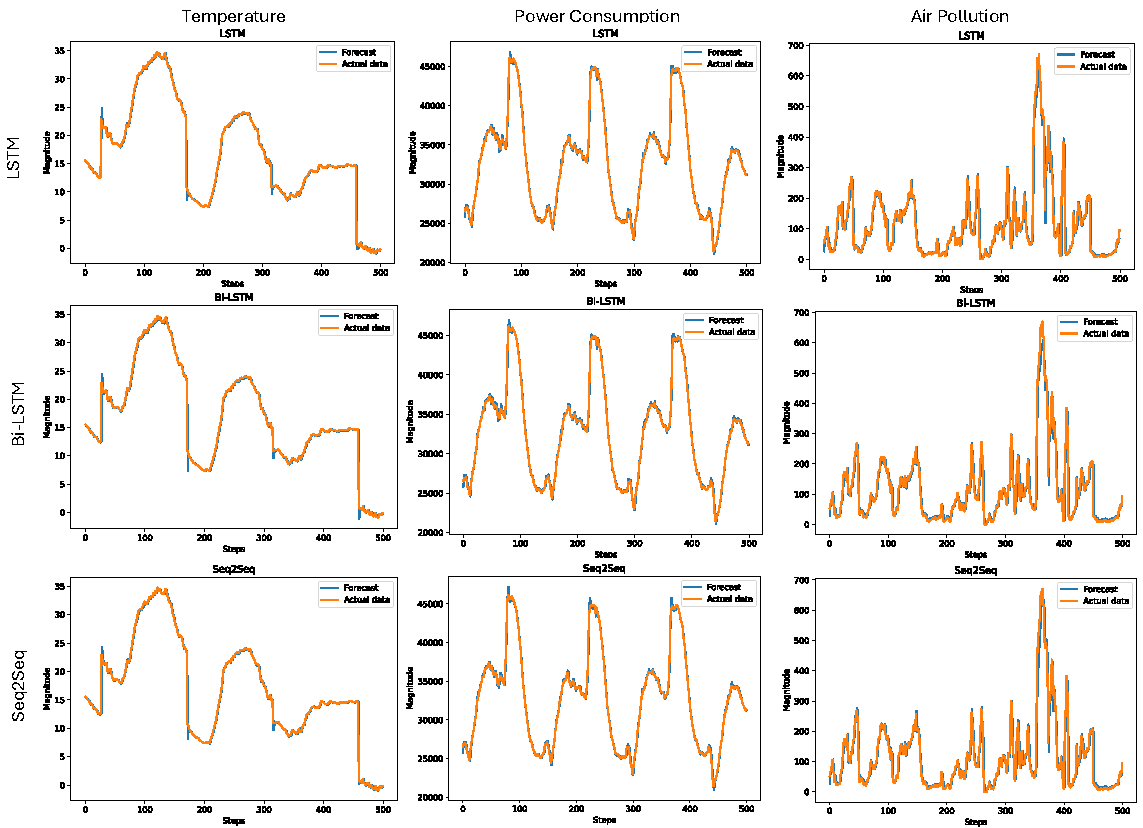
\includegraphics[scale=0.6]{sn-article-template/modern.pdf}
	\end{center}
	\caption{Plots: comparison between predicted values vs. ground truth for three modern techniques (LSTM, Bi-LSTM, and Seq2Seq) across three datasets.}
	\label{fig:modern}
\end{figure}


\textbf{State-of-Art Transformers.} We also implemented the Transformers model, a state-of-the-art architecture with a self-attention mechanism. To ensure consistency, we used the same hyperparameters as the modern techniques, as shown in Table \ref{tab:hyperparams}. Based on the prediction vs. actual plots in Figure \ref{fig:trans} and the metrics in Table \ref{tab:trans_metric}, the Transformers model outperforms the classical models but does not exceed the performance of the three modern techniques. This suggests that for these datasets, the complex Transformers architecture may not be necessary for optimal performance.
\begin{table}[h]
\centering
\begin{tabular}{@{}lccc@{}}
\toprule
\textbf{}               & \textbf{MSE} & \textbf{RMSE} & \textbf{MAE} \\ \midrule
% \textbf{Transformers}    &              &               &              \\
Temperature             & 0.000599     & 0.024466      & 0.016530     \\
Power consumption       & 0.000467     & 0.021602      & 0.015685     \\
Air pollution           & 0.001370     & 0.037011      & 0.019526     \\ \bottomrule
\end{tabular}
\caption{Performance metrics for Transformers model. Both prediction and ground truth are normalized using the Equation \ref{nomalize}.}
\label{tab:trans_metric}
\end{table}
\begin{figure}[H]
	\begin{center}
		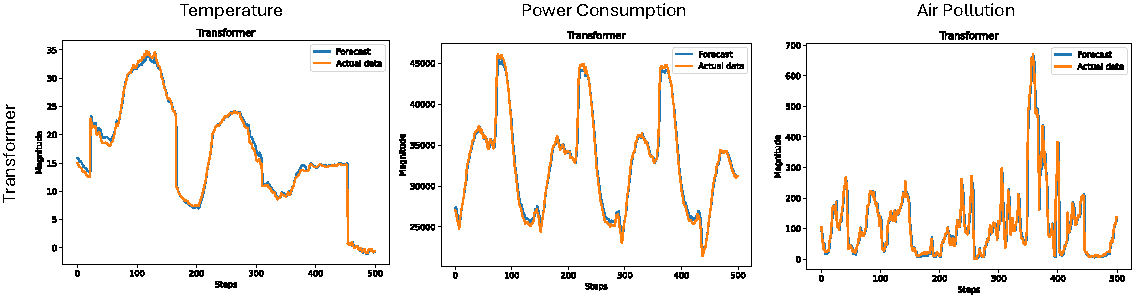
\includegraphics[scale=0.6]{sn-article-template/trans.pdf}
	\end{center}
	\caption{Plots for predicted values vs. ground truth for Transformers across three datasets.}
	\label{fig:trans}
\end{figure}

\section{Conclusion}
In this study, we evaluated the performance of four classical models (AR, MA, ARMA, ARIMA), three modern techniques (LSTM, BiLSTM, Seq2Seq), and a state-of-the-art Transformers model on three publicly available datasets. Our findings indicate that while the classical models were relatively simple, both modern techniques and the Transformers consistently outperformed them. Among the deep learning models, LSTM, with its simple architecture, achieved the lowest MSE, suggesting that even basic deep learning models can effectively handle the data in these cases.

However, this study has some limitations. For the classical models, we used relatively simple configurations based on available information, which may not reflect their optimal performance. A more extensive exploration of the model configurations could yield better results. Additionally, while Optuna was employed for hyperparameter tuning, we constrained the maximum order and number of trials, and relaxing these limits could lead to improved model selection.

For the modern techniques and Transformers, all models were trained with a fixed sequence length and a common set of hyperparameters, which may not be optimal for every model or dataset.

Future work could involve implementing Seasonal Autoregressive Integrated Moving Average (SARIMA) \cite{box2015time} models to better capture the seasonality present in the datasets. Additionally, applying advanced techniques such as the Box-Jenkins \cite{box2015time} methodology and exploring other model variations could provide a more comprehensive performance comparison. By addressing these limitations and exploring alternative approaches, we aim to refine our findings and broaden the scope of this research.




\bibliography{sn-bibliography}


\end{document}
